\subsection{Ordenamiento de Mo}

\begin{frame}[fragile]
  \frametitle{El truco de Mo}

  Fijate que realmente podemos extender y achicar el rango de la consulta:

\begin{lstlisting}
void metesaca(int j) {
    if (tengo[j]) {
        <saca>
    } else {
        <mete>
    }
    tengo[j] = !tengo[j];
}
\end{lstlisting}

  O sea, si tenemos en algún momento acumulado el intervalo \([l, r)\), podemos \emph{metesacar} (\(l-1\), \(l\), \(r-1\) o \(r\)) para obtener los intervalos \([l-1, r)\), \([l+1, r)\), \([l, r-1)\) o \([l, r+1)\).
\end{frame}

\begin{frame}
  \frametitle{El truco de Mo: movimiento en el plano}

  Si pensamos en el intervalo \([l, r)\) como un punto \((l,r)\) en el plano, podemos movernos hacia arriba, abajo, izquierda o derecha.

  \vspace{0.75em}

  A medida que nos movemos por el plano, podemos llegar a posiciones que se corresponden con las consultas que tenemos que hacer.

  En esos puntos, podemos guardar el valor acumulado para obtener la respuesta de la consulta.

  \vspace{0.75em}

  Resulta posible elegir un orden de movimiento tal que el costo total sea \(O((N + Q)\sqrt{N})\).
\end{frame}

\begin{frame}
  \centering
  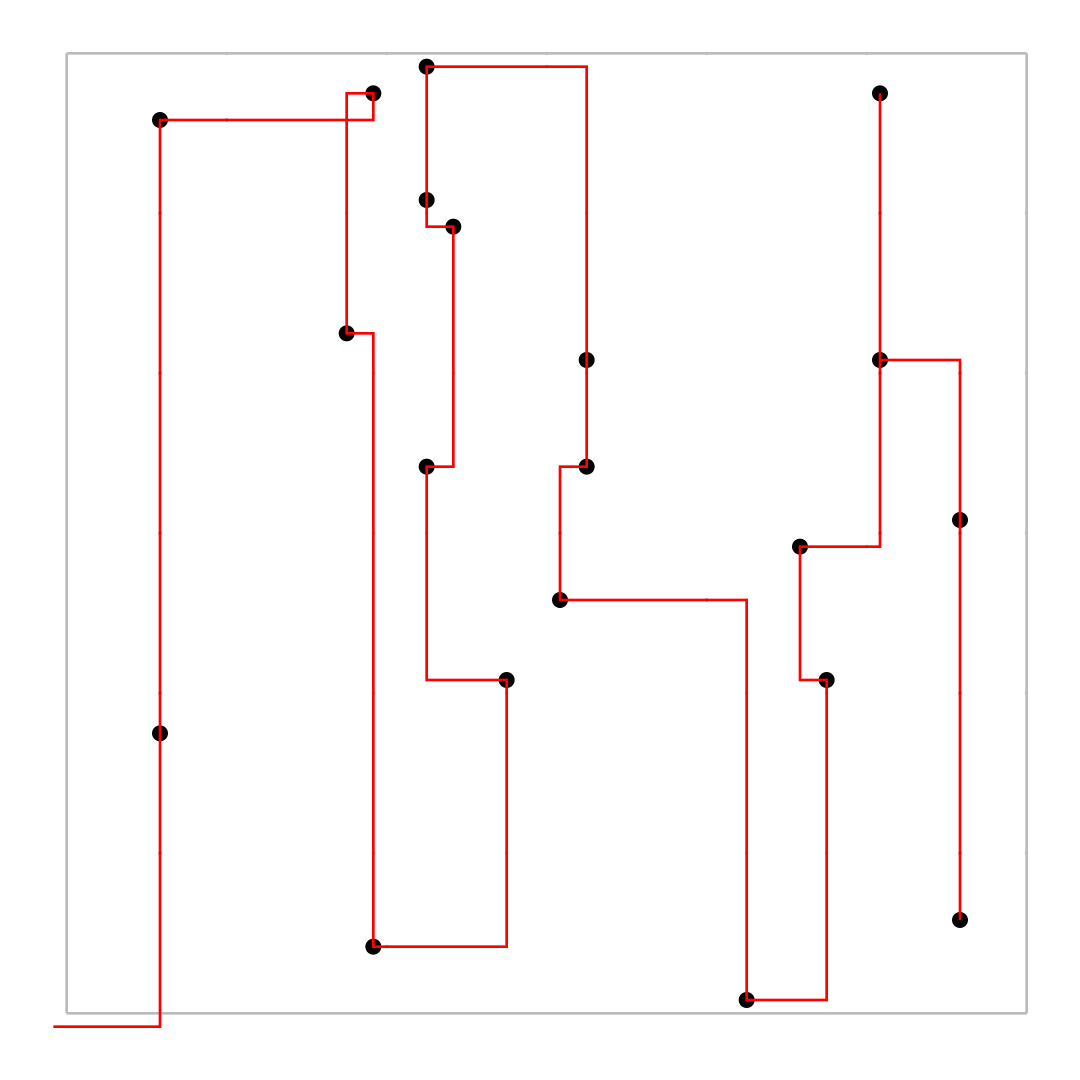
\includegraphics[height=0.85\textheight,keepaspectratio]{fotos/path-clean.png}
\end{frame}

\begin{frame}
  \frametitle{El truco de Mo: complejidad}

  Partimos el plano en cuadrados de \(\sqrt{N} \times \sqrt{N}\) y recorremos los cuadrados en zig zag.

  \vspace{0.75em}

  Pasar de cada punto al siguiente cuesta \(O(\sqrt{N})\) si está en el mismo bloque. En total sobre todos los puntos es \(O(Q\sqrt{N})\).

  \vspace{0.75em}

  Podemos considerar por separado el caso de cambiar de bloque.

  En total hay \(O(N)\) bloques, y moverse de uno a otro cuesta \(O(\sqrt{N})\). En total es \(O(N\sqrt{N})\).

  \vspace{0.75em}

  Entonces, el costo total es \(O((Q + N)\sqrt{N})\).
\end{frame}
